\label{sec:model_reference_control}
\section{Introduction}
The first part of this chapter is a summary of the work presented in \cite{Data-driven_model_reference_control}. From section \ref{sec:freq_domain_translate} and on, improvements are made to the existing methods.

\section{Problem statement}
% Firstly, I will assume to be working with a SISO system $G(\Omega)$. $\Omega$ can either be $s$ or $z^{-1}$.
% \begin{equation*}
%     \Omega = \begin{cases}
%         s & \text{if working in continuous-time (CT)} \\
%         z^{-1} & \text{if working in discrete-time (DT)} 
%     \end{cases}
% \end{equation*}
The first assumption that is made is that $G(\Omega)$ is stable and minimum-phase. It is also possible to extend this theory to unstable nonminimum-phase systems. This will be done later in section \ref{sec:unstable}.

The system is controlled by an unknown controller $K(\Omega,\rho)$ in closed loop (CL). This is shown graphically in figure \ref{fig:closed_loop_system}.

\begin{figure}[H]
    \centering
    \includegraphics[width = 0.65\textwidth]{figures/closed_loop_system.pdf}
    \caption{Closed loop system.}
    \label{fig:closed_loop_system}
\end{figure}

The transfer function from the reference $r$ to the output $y$ is given by
\begin{equation*}
    \text{CL}(\Omega) = \frac{K(\Omega,\rho) G(\Omega)}{1 + K(\Omega,\rho) G(\Omega)}
\end{equation*}
$\rho = \begin{bmatrix}
        \rho_1 & \ldots & \rho_{n_{\rho}}
\end{bmatrix}^T$ is a vector containing the optimization parameters. In this work $K(\Omega,\rho)$ is linear in the parameters.
\begin{equation}
    K(\Omega,\rho) = \beta(\Omega) \rho
    \label{eq:linear_in_the_parameters}
\end{equation}
with $\beta(\Omega)$ being a row vector with $n_\rho$ elements.
The idea of model reference control, is to get the closed loop system ``as close'' as possible to a used-defined reference system $M(\Omega)$.
\begin{equation*}
    M(\Omega) \approx \frac{K(\Omega,\rho) G(\Omega)}{1 + K(\Omega,\rho) G(\Omega)}
\end{equation*}
$M(\Omega)$ is assumed to be a stable causal LTI system. This criterion can be quantified by using the 2-norm of a transfer function.
\begin{equation}
    J_{mr}(\rho) =  \Big|\Big|F(\Omega) \Big[M(\Omega)-\frac{K(\Omega,\rho) G(\Omega)}{1 + K(\Omega,\rho) G(\Omega)}\Big]  \Big|\Big|_2^2 
    \label{eq:Jmr}
\end{equation}
$F(\Omega)$ is a user-defined weighing filter that can be chosen to highlight specific frequencies. The 2-norm of a SISO system is defined differently for CT and DT systems. For CT systems it is
\begin{equation*}
    ||H(s)||_2^2 = \frac{1}{2\pi} \int_{-\infty}^{+\infty} |H(j\omega)|^2 d\omega
\end{equation*}
and for DT systems it is
\begin{equation*}
    ||H(z^{-1})||_2^2 = \frac{1}{2\pi} \int_{-\pi}^{\pi} |H(e^{j\omega})|^2 d\omega
\end{equation*}

\newpage
 \section{Convex cost}
One problem with the use of (\ref{eq:Jmr}) as a cost function is that it is not convex.
In order to solve this, we must first define the ideal controller $K^*(\Omega)$ as
\begin{equation}
    K^*(\Omega) = \frac{M(\Omega)}{G(\Omega)(1-M(\Omega))}
    \label{eq:Kstar_def}
\end{equation}
This definition ensures that the closed loop system is equal to the reference system by construction.
\begin{equation*}
    \frac{K^*(\Omega) G(\Omega)}{1 + K^*(\Omega) G(\Omega)} = M(\Omega)
\end{equation*}
Note that it is possible that $K^*$ is not realizable i.e. 
\begin{equation*}
    \nexists \rho \text{ such that } K(\Omega,\rho) = K^*(\Omega)
\end{equation*}

Next, both terms in (\ref{eq:Jmr}) can be put under the same denominator.
\begin{equation*}
    M(\Omega)-\frac{K(\Omega,\rho) G(\Omega)}{1 + K(\Omega,\rho) G(\Omega)} = \frac{M(\Omega)-(1-M(\Omega))K(\Omega,\rho) G(\Omega)}{1 + K(\Omega,\rho) G(\Omega)}
\end{equation*}
The sensitivity function is approximated by the ideal sensitivity function. The validity of this approximation should be verified afterwards.
\begin{equation*}
    \frac{1}{1 + K(\Omega,\rho) G(\Omega)} \approx \frac{1}{1 + K^*(\Omega) G(\Omega)} = \frac{1}{1+\frac{M(\Omega)}{1-M(\Omega)}} = 1-M(\Omega)
\end{equation*}
This leads to the definition of the convex cost function.
\begin{equation}
\boxed{
    J(\rho) =  \Big|\Big|F(\Omega)(1-M(\Omega)) \Big[M(\Omega)-(1-M(\Omega))K(\Omega,\rho) G(\Omega)\Big]  \Big|\Big|_2^2 
    \label{eq:J}
}
\end{equation}
Of course, not all forms of $K(\Omega,\rho)$ will make this cost function convex. However, this is the case when $K(\Omega,\rho)$ is linear in the parameters (\ref{eq:linear_in_the_parameters}). Note that the cost is minimized for the ideal controller if the ideal controller is realizable.
\begin{equation*}
    K(\rho^*,\Omega) = K^*(\Omega) \Longrightarrow J(\rho^*) = 0
\end{equation*}

\section{Other cost functions}
We can devise many other cost functions that solve this problem. An example is the following.
\begin{equation*}
    J_K(\rho) = ||K^*(\Omega)-K(\Omega,\rho)||_2^2
\end{equation*}
This cost function minimizes the square of the difference between the actual controller $K(\Omega,\rho)$ and the ideal controller $K^*(\Omega)$. If $K(\Omega,\rho)$ is linear in the parameters, then this is just a simple least squares regression. However, this is not the same as optimizing $\rho$ to the cost function (\ref{eq:J}) and will result in a different outcome. \textcolor{red}{In fact, it can be shown that (\ref{eq:J}) is a weighted least squares regression problem. By using (\ref{eq:Kstar_def}) we get
\begin{equation*}
    M(\Omega) = G(\Omega) (1-M(\Omega)) K^*(\Omega)
\end{equation*}
Using this expression in (\ref{eq:J}) results in
\begin{align*}
    J(\rho) & =  \Big|\Big|F(\Omega)(1-M(\Omega)) \Big[G(\Omega) (1-M(\Omega)) K^*(\Omega)-(1-M(\Omega))K(\Omega,\rho) G(\Omega)\Big]  \Big|\Big|_2^2 \\
    &= \Big|\Big|F(\Omega)(1-M(\Omega))^2 G(\Omega) \Big[ K^*(\Omega)-K(\Omega,\rho) \Big]  \Big|\Big|_2^2 
\end{align*}
Note that that $J(\rho)$ depends on $G(\Omega)$ both directly and indirectly as $K^*$ also depends on $G(\Omega)$. No expression for $G(\Omega)$ is known in the data-driven approach and it will therefore have to be estimated.}
This shows that the choice of the cost function is an important part of optimization and must be done with care.

\section{Correlation-based approach}
\label{sec:corr_based_approach}
As $G(\Omega)$ is not known in (\ref{eq:J}), the authors of \cite{Data-driven_model_reference_control} propose the correlation-based approach. They give algorithms for periodic and arbitrary excitations. Here we will focus on their equations concerning periodic excitations. We will also restrict this section to DT systems ($\Omega = z^{-1}$), as they have done in their paper.

One thing to note, is that all the equations in \cite{Data-driven_model_reference_control} are written in the TD. These will be translated to the FD in section \ref{sec:freq_domain_translate}. The reader is recommended to not to spend too much time trying to understand the definitions in this section as they will make more sense in the next section.

\paragraph{Model}
First it is assumed that the output of the DT system is perturbed by some noise $v(n)$.
\begin{equation}
    y(n) = G(q^{-1}) u(n) + v(n)
    \label{eq:model_TD}
\end{equation}
with $q^{-1}$ being the backshift operator: $q^{-1} x(n) = x(n-1)$. $N$ denotes the period of the input.
\begin{equation}
    u(n) = u(n+N)
    \label{eq:periodicity_u}
\end{equation}
The additive noise is modelled as DT filtered white noise.
\begin{equation*}
    v(n) = S_v(q^{-1}) e_v(n) \,, e_v(n) \text{ with } \mathbb{E}\{e_v(n)\} = 0 \text{ and } \mathbb{E}\{e_v(n)^2\} = \sigma^2
\end{equation*}

\paragraph{Error signal}
Then a new quantity $\epsilon(n,\rho)$ is defined \cite[eq. (15)]{Data-driven_model_reference_control}.
\begin{align*}
    \epsilon(n,\rho) &= M(q^{-1}) u(n) - K(q^{-1},\rho) (1-M(q^{-1})) y(n) \\
    &= [M-K(\rho) (1-M) G ] u(n) - K(\rho) (1-M) v(n)
\end{align*}
In the second row the operators $q^{-1}$ are left out for clarity. \textcolor{red}{Notice that when $K(\rho) = K^*$, the first term cancels out.
\begin{equation*}
	\epsilon^*(n) = -K^*(1-M)v(n)
\end{equation*}
Thus $\epsilon(n,\rho)$ is uncorrelated with $u(n)$ when $\rho = \rho^*$. The main idea behind the correlation-based approach is to tune the parameters $\rho$ such that $\epsilon(n,\rho)$ becomes uncorrelated with $u(n)$. Note however that this reasoning only holds if $K^*$ is realizable with the proposed controller scheme $K(\rho)$. If $K^*$ is not realizable, then the first term $[M-K(\rho) (1-M) G ]$ will not be zero when replacing $K(\rho)$ with the optimal controller and $\epsilon(n,\rho)$ will still be correlated to $u(n)$.
}

\paragraph{Input filtering}
Additionally, the filter $W$ is defined \cite[eq. (41)]{Data-driven_model_reference_control}
\begin{align*}
    W(e^{-j\omega_k}) &= \frac{F(e^{-j\omega_k})(1-M(e^{-j\omega_k}))}{S_{UU}(e^{-j \omega_k})} \\
    \omega_k &= \frac{2\pi k}{N} \,,\quad k=0,\ldots,N-1
\end{align*}
$S_{UU}(e^{-j \omega_k})$ is the DFT of the autocorrelation of u(n) \cite[eqs. (38) and (39)]{Data-driven_model_reference_control}.
\begin{align}
    R_{uu}(\tau) &= \frac{1}{N}\sum_{n=0}^{N-1} u(n-\tau) u(n) \label{eq:Rutau}\\
    S_{UU}(e^{-j \omega_k}) &=  \sum_{\tau=0}^{N-1} R_{uu}(\tau) e^{-j \tau \omega_k}\label{eq:Suu}
\end{align}
If the system is in steady state, $u(n-\tau)$ is known for negative time indices by using (\ref{eq:periodicity_u}). If the experiment starts with zero initial conditions, then $u(n-\tau) = 0$ for $n-\tau < 0$.

The filter $W$ is applied to the input $u(n)$. As is remarked at the end of \cite[Sec. 4.4]{Data-driven_model_reference_control}, if a parametric representation of $S_{UU}(q^{-1})$ is known, this filter can be applied in the TD.
\begin{equation*}
    u_W(n) = W(q^{-1}) u(n)
\end{equation*}
Note that this can be problematic if $S_{UU}(q^{-1})$ has zeros that are not on the unit circle, as the filter $W(q^{-1})$ will then be unstable. More information concerning this is given in appendix \ref{appendix:W_filtering}.

\paragraph{Correlation criterion}
Then, the crosscorrelation between between $u_W(n)$ and $\epsilon(n,\rho)$ is calculated.
\begin{equation}
    R_{u_W \epsilon}(\tau,\rho) = \frac{1}{N\!P} \sum_{n=0}^{N\!P-1} u_W(n-\tau) \epsilon(n,\rho)
    \label{eq:RuWepstau}
\end{equation}
with $P$ being the number of periods measured. Note that as in (\ref{eq:Rutau}), $u_W(n-\tau)$ can be found by using (\ref{eq:periodicity_u}) if the system is in steady state. If the system starts off in zero initial conditions, $u_W(n-\tau) = 0$ for $n-\tau < 0$.

The correlation criterion $J_{N\!P,l_1}(\rho)$ can then be defined.
\begin{equation}
\boxed{
    J_{N\!P,l_1}(\rho) = \sum_{\tau=-l_1}^{l_1} R_{u_W \epsilon}^2(\tau,\rho)
}
\label{eq:JNl1}
\end{equation}
with $l_1 \leq N/2$ being a parameter that can be chosen by the user. The idea behind this parameter $l_1$ is discussed in detail in section \ref{sec:parseval}. It is then proven in \cite[Appendix II]{Data-driven_model_reference_control} that (\ref{eq:JNl1}) converges to (\ref{eq:J}) for $N,P \rightarrow \infty$ with probability 1 under certain conditions.
\begin{equation*}
    \lim_{N,P\rightarrow \infty} J_{N\!P,l_1}(\rho) = J(\rho) \,,\, \text{w.p. } 1
\end{equation*}
However, for finite data, it is proven that the estimator is biased \cite[eq. (37)]{Data-driven_model_reference_control}
\begin{equation}
    \mathds{E}\{J_{N\!P,l_1}(\rho)\} \approx \Tilde{J}_{N\!P,l_1}(\rho) + \frac{\sigma^2 (2l_1+1)}{2\pi N\!P} \int_{-\pi}^\pi \frac{|1-M|^4|K(\rho)|^2|S_v|^2|F|^2}{S_{UU}(e^{-j\omega})} d\omega
    \label{eq:bias_on_JNl1}
\end{equation}
with $\Tilde{J}_{N\!P,l_1}(\rho)$ being the control criterion in the absence of noise. A proof of this is given in section \ref{sec:bias}.

\section{Translation to frequency domain}
\label{sec:freq_domain_translate}
In this section the results from the previous section will be translated to the FD. Here we will show that a nonparametric estimate of the system $G(\Omega)$ is actually hidden in the mathematics. Thus, even though the parametric modeling step is skipped, there is still a nonparametric model.

\subsection{Disadvantages of TD}
There are some disadvantages of working in the TD. Here are some that are relevant to this subject.
\begin{itemize}
    \item TD filtering can only be done easily if the underlying system is a DT system.
    \item The filtering of $u(n)$ with $W(q^{-1})$ can only be performed in the TD if a parametric representation of $S_{UU}(q^{-1})$ is known and if $S_{UU}(q^{-1})$ only has zeros on the unit circle. (see appendix \ref{appendix:W_filtering}).
    \item If the system starts with zero initial conditions or in steady state, then the transient response can be taken into account, as knowledge of the input and output signals are known before they are applied. This makes it possible to calculate (\ref{eq:Rutau}) and (\ref{eq:RuWepstau}) for $n-\tau < 0$. However, if the system does not start with zero initial conditions or in steady state, this approach will not work and the transient term will not be suppressed.
\end{itemize}
These problems can be solved by working in the FD. To address the first point: FD methods can also handle CT systems. For the second point: a convolution in the TD can explode when the system is unstable. However, this is not a problem in the FD as a convolution in the TD becomes a simple multiplication in the FD. Finally, for the third point: the robust LPM (see section \ref{sec:LPM}) is able to estimate nonparametrically the frequency response function (FRF) from noisy input-output data, while suppressing the transient term.


% For the remainder of this section, a simplified approach to estimating the FRF is used to illustrate how the TD algorithm outlined in the beginning of this section can be translated to the FD.

% First, the DFT of the input u(n) and output y(n) is defined. As before, I assume that $u(n)$ is periodic with a period of $N$ samples. $n_p$ periods of $y(n)$ are measured.

% \begin{align*}
%     U^{(m)}(k) &= \text{DFT}\{ u^{(m)}(n) \}(k) \,,\, k = 0,\ldots,N-1\\
%     Y^{(m)}(k) &= \text{DFT}\{ y^{(m)}(n) \}(k)  \,,\, k = 0,\ldots,N-1
% \end{align*}
% with the superscript $(m)$ denoting the period ($m = 1,\ldots,n_p$). Working with periodic data allows for taking the mean of the spectra over the DFT bins.
% \begin{align*}
%     U(k) &= \frac{1}{P} \sum_{m=1}^{P} U^{(m)}(k) \\
%     Y(k) &= \frac{1}{P} \sum_{m=1}^{P} Y^{(m)}(k)
% \end{align*}
% The auto power spectrum of $u(n)$ is simply 
% \begin{equation*}
%     S_{UU}(\Omega_k) = U(k) \overline{U(k)}
% \end{equation*}
% with $\overline{\bullet}$ denoting the complex conjugate operator. FD methods are not restricted to DT systems. So $\Omega_k$ is defined as:

% \begin{equation*}
%     \Omega_k = \begin{cases}
%         j 2 \pi k F_s/N & \text{if working in continuous-time (CT)} \\
%         e^{j 2 \pi k/N}& \text{if working in discrete-time (DT)} 
%     \end{cases}
% \end{equation*}
% $F_s$ is the sampling frequency.
\subsection{Nonparametric estimate}
By translating the formulas of section \ref{sec:corr_based_approach} to the FD, it will become immediately apparent that a nonparametric estimate is being calculated. The first step in translating the problem from the TD to the FD is to use Parseval's theorem. According to Parseval's theorem, the sum of squares in the TD is equivalent to the sum of the norms squared in the FD. The cost function (\ref{eq:JNl1}) represents a sum of squares in the TD. Parseval's theorem will be discussed in greater detail in section \ref{sec:parseval}.

Now, instead of calculating $\epsilon(n,\rho)$ in the TD, it can be calculated in the FD. Note that this also makes the computations less intensive, as a convolution in the TD becomes a multiplication in the FD. As the input to the system is assumed to be periodic, the frequencies $\Omega_k$ will correspond to the DFT bins $kP$.
\begin{equation*}
    E(kP,\rho) = M(\Omega_k) U(kP) - K(\Omega_k,\rho) (1-M(\Omega_k)) Y(kP)
\end{equation*}
Applying the filter $W$ on $u(n)$ can also be done in the FD.
\begin{equation*}
    U_W(kP) = W(\Omega_k) U(kP)
\end{equation*}
with
\begin{equation*}
    W(\Omega_k) = \frac{F(\Omega_k)(1-M(\Omega_k))}{S_{UU}(e^{-j \omega_k})}
\end{equation*}
The denominator $S_{UU}(e^{-j \omega_k})$ is proportional to $U(kP)\overline{U(kP)}$.
\begin{equation}
S_{UU}(e^{-j \omega_k}) = N U(kP)\overline{U(kP)}
\label{eq:Suu=NUU}
\end{equation}
This equivalence is proven in appendix \ref{appendix:DFT_cross}. Then, the cross-power spectrum between $\epsilon(n,\rho)$ and $u_W(n)$ is also calculated in the FD by doing a simple multiplication.
\begin{equation}
    S_{U_W\!E}(\Omega_k,\rho) = N U_W(kP) \overline{E(kP,\rho)}
    \label{eq:RWE_FD}
\end{equation}
Expanding (\ref{eq:RWE_FD}) makes the link to the cost function (\ref{eq:J}) immediately apparent.
\begin{align}
    S_{U_W\!E}(\Omega_k,\rho) &= U(kP) \frac{F(1-M)}{U(kP)\overline{U(kP)}}  \overline{ \big(M U(kP) - K(\rho) (1-M) Y(kP) \big)} \label{eq:PhiUwepsilon_FD}\\
    &= F (1-M) \overline{\big( M - K(\rho) (1-M)\hat{G}(\Omega_k) \big)}
    \label{eq:cross-power_in_FD}
\end{align}
with 
\begin{equation}
    \hat{G}(\Omega_k) = \frac{Y(kP) \overline{U(kP)}}{U(kP) \overline{U(kP)}} = \frac{Y(kP)}{U(kP)}
    \label{eq:Ghat=YU/UU}
\end{equation}
The index $\Omega_k$ was left out in $F$, $M$ and $K$ for clarity.
$\hat{G}(\Omega_k)$ is a nonparametric estimate of the system. If $\hat{G}$ is replaced by the actual system $G$, then $S_{U_W\!E}(\Omega_k,\rho)$ is exactly the quantity being integrated over in (\ref{eq:J}).

\newpage
Thus, a nonparametric estimate of the system $\hat{G}$ can be found, followed by calculating the cost function in the FD.
\begin{equation}
\boxed{
    J_N(\rho) = \frac{1}{|\kexc|}\sum_{k \in \kexc} \Big|H(\Omega_k,\rho)\Big|^2
\label{eq:JFD}
}
\end{equation} 
with $\kexc$ being the set of excited DFT bins, $|\kexc|$ being the cardinality of this set and
\begin{equation}
    H(\Omega_k,\rho) = F(\Omega_k)(1-M(\Omega_k)) \Big[M(\Omega_k)-(1-M(\Omega_k))K(\Omega_k,\rho) \hat{G}(\Omega_k)\Big]
\end{equation}
Proceeding in this way, we can be much more flexible with the manner in which we estimate the FRF nonparametrically. Let's take a closer look at the nonparametric estimator that is hidden inside the formulas of the TD.
\begin{equation*}
    \hat G(\Omega_k) = \frac{Y(kP)}{U(kP)}
\end{equation*}
Now, let's separate $y(n)$ into its P periods $y^{(p)}(n)$.
\begin{equation*}
    y^{(p)}(n) = y(n+pP) \,,\quad p = 0,\ldots,P-1
\end{equation*}
We can also define the DFT for every one of the periods.
\begin{equation*}
    Y^{(p)}(k) = \sum_{n=0}^{N-1} y^{(p)}(n) e^{-j2\pi kn/N} \,,\quad p = 0,\ldots,P-1
\end{equation*}
With these definitions we can get a better understanding of what $Y(kP)$ represents.
\begin{align*}
    Y(kP) &= \sum_{n=0}^{N\!P-1} y(n) e^{-j2\pi (kP) n/(N\!P)}\\
    &= \sum_{p=0}^{P-1}  \sum_{n=0}^{N-1} y(n+pP) e^{-j2\pi kn/N} = \sum_{p=0}^{P-1} Y^{(p)}(k)
\end{align*}
Thus, the nonparametric estimate becomes
\begin{equation*}
    \hat G(\Omega_k) = \frac{\frac{1}{P}\sum_{p=0}^{P-1}  Y^{(p)}(k)}{\frac{1}{P}\sum_{p=0}^{P-1}  U^{(p)}(k)}
\end{equation*}
This is a consistent estimator for the model (\ref{eq:model_TD}). Indeed, if we translate (\ref{eq:model_TD}) to the FD we obtain
\begin{equation*}
    Y^{(p)}(k) = G(\Omega_k) U^{(p)}(k) + V^{(p)}(k) \,,\quad p = 0,\ldots,P-1
\end{equation*}
Given that the input is periodic $U^{(p)}(k) = U_0(k)$, we get
\begin{equation*}
    \hat G(\Omega_k) = \frac{\frac{1}{P}\sum_{p=0}^{P-1} \Big [ G(\Omega_k) U_0(k) + V^{(p)}(k) \Big ]}{U_0(k)} = G(\Omega_k) + \frac{1}{U_0(k)} \frac{1}{P}\sum_{p=0}^{P-1} V^{(p)}(k)
\end{equation*}
The output noise is assumed to be Gaussian white noise, which means that $\mathbb{E}\{V(k)\}=0$. Taking the limit for $P \rightarrow \infty$ gives
\begin{equation*}
    \lim_{P \rightarrow \infty} \hat G(\Omega_k) = G(\Omega_k) + \frac{1}{U_0(k)} \mathbb{E}\{V(k)\} = G(\Omega_k) \,,\, \text{w.p. } 1
\end{equation*}
The law of large numbers for independent experiments is used in the first equation. The estimator is also consistent if the measurement of the input is noisy.
\begin{equation*}
    U^{(p)} = U_0(k) + N_U^{(p)}(k)
\end{equation*}

\newpage
\section{Parseval's theorem}
\label{sec:parseval}
Parseval's theorem is very simple: the energy of the signal in the TD is the same as the energy of the signal in the FD.
\begin{equation}
    \sum_{n=0}^{N-1} x(n)^2 = N \sum_{k=0}^{N-1} |X(k)|^2
    \label{eq:parseval_theorem}
\end{equation}
with $X(k) = \text{DFT}\{x(n)\}$. The factor $N$ is specific to the definition of the DFT that is used in this work and will be different if another definition is used.

The cost function in the FD (\ref{eq:JFD}) is also the sum of squares.
\begin{equation*}
    J_N(\rho) = \frac{1}{N} \sum_{k=0}^{N-1} |H(\Omega_k,\rho)|^2
\end{equation*}
According to Parseval's theorem, the above sum is equivalent to a sum of squares in the TD.
\begin{equation*}
    J_N(\rho) = \sum_{n=0}^{N-1} h(n,\rho)^2
\end{equation*}
with $h(n,\rho)$ being the IDFT of $H(\Omega_k,\rho)$. If $N \rightarrow \infty$, $h(n,\rho)$ is the impulse response of the system $H(\Omega,\rho)$. The trick that the authors use in \cite{Data-driven_model_reference_control} is the fact that the impulse response of a stable system will fade away after some time.
\begin{equation*}
    \exists l_1 \text{ such that } h(n) \approx 0 \text{ for } n > l_1
\end{equation*}
Applying this approximation to the cost function gives
\begin{equation}
    J_N(\rho) \approx  \sum_{n=0}^{l_1} h(n,\rho)^2
    \label{eq:Japprox_impulse_response}
\end{equation}


\paragraph{Example}
Let's take a very simple first order system.
\begin{equation}
    H(z^{-1}) = \frac{0.2 z^{-1}}{1 - 0.8 z^{-1}}
    \label{eq:parseval_example_H}
\end{equation}
The impulse response of this system for the first 51 samples is plotted in figure \ref{fig:parseval_signal}. Additionally, the red dotted line shows the impulse response with a bit of additive Gaussian white noise.

\begin{figure}[H]
    \centering
    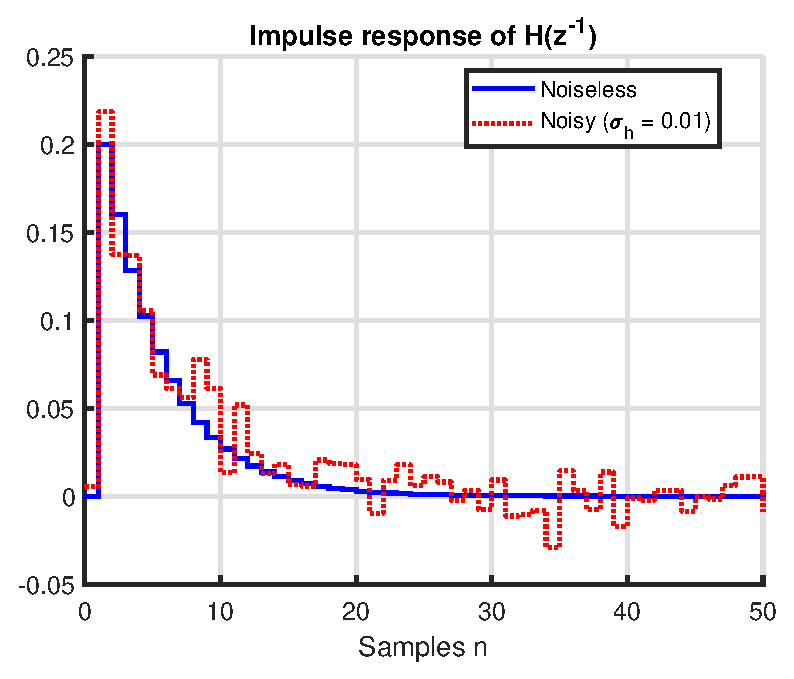
\includegraphics[width = 0.65 \textwidth]{figures/parseval_signal.eps}
    \caption{Impulse response of (\ref{eq:parseval_example_H}) with and without additive Gaussian white noise.}
    \label{fig:parseval_signal}
\end{figure}

The approximate energy of the signal in the TD $\sum_{n=0}^{l_1} h(n,\rho)^2$ is plotted in figure \ref{fig:parseval_energy} (blue full line). It quickly converges to the energy of the signal in the FD $\frac{1}{51} \sum_{k=0}^{50} |H(k)|^2$. This is also the case for the noisy signal (dotted red line); it converges to its energy in the FD. Ideally however, we would like the energy in the noisy case to be as close to the actual, noiseless energy. This is not the case; there is a certain bias. In this case, taking $l_1 = 10$, would result in less bias, while still keeping the information that is needed. This can also be seen in figure \ref{fig:parseval_signal}: the impulse response after $n = 10$ is at or below noise level. Thus the impulse response after $n = 10$ does not contain much useful information and will only contribute to a biased cost function.

\begin{figure}[H]
    \centering
    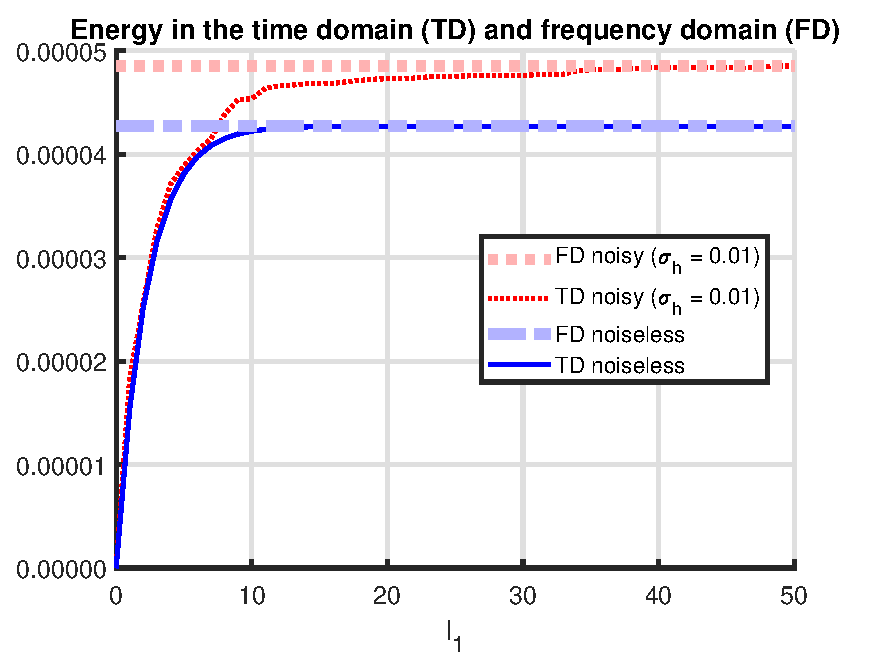
\includegraphics[width = 0.65 \textwidth]{figures/parseval_energy.eps}
    \caption{Energy of the signal in the TD and the FD (divided by $N$).}
    \label{fig:parseval_energy}
\end{figure}

In \cite{Data-driven_model_reference_control}, $l_1$ has a slightly different interpretation. As it can be seen in (\ref{eq:RuWepstau}), the sum goes from $-l_1$ to $l_1$. This is because the sum is taken over the crosscorrelation of $u_W$ and $\epsilon$. The crosscorrelation is meaningful for both positive and negative indices, which is why the sum also extends into negative values of $\tau$. The impulse response for negative indices is zero for causal systems, which is why the sum starts at $n = 0$ in (\ref{eq:Japprox_impulse_response}).

\newpage
\section{Bias}
\label{sec:bias}
Let's quantify the bias that was discussed in the previous section. The results will be very close to (\ref{eq:bias_on_JNl1}). Let's assume that the input is a periodic signal that is excited at all the DFT frequencies. The output is perturbed by filtered white noise.
\begin{equation*}
    Y^{(p)}(k) = G(\Omega_k)U_0(k) + S_v(\Omega_k) V^{(p)}(k)
\end{equation*}
with $\mathbb{E}\{V^{(p)}(k)\} = 0$ and $\mathbb{E}\{|V^{(p)}(k)|^2\} = \sigma^2/N$. The nonparametric estimate of the FRF is
\begin{equation*}
    \hat G(\Omega_k) = \frac{\frac{1}{P}\sum_{p=0}^{P-1}  Y^{(p)}(k)}{\frac{1}{P}\sum_{p=0}^{P-1}  U^{(p)}(k)} = G(\Omega_k) + \frac{1}{U_0(k)} \frac{1}{P}\sum_{p=0}^{P-1} S_v(\Omega_k) V^{(p)}(k)
\end{equation*}
The statistical properties of this estimator are
\begin{align*}
    \mathbb{E}\{\hat G(\Omega_k)\} &= G(\Omega_k)\\
    \mathbb{E}\{|\hat G(\Omega_k)|^2\} &= |G(\Omega_k)|^2 + \frac{1}{|U_0(k)|^2}\frac{|S_v(\Omega_k)|^2 \sigma^2}{NP}\\
    &= |G(\Omega_k)|^2 + \frac{1}{N\!P}\frac{|S_v(\Omega_k)|^2 \sigma^2}{|U_0(k)|^2}
\end{align*}
$|S_v(\Omega_k)|^2 \sigma^2$ quantifies the power of the noise at the $k$-th DFT bin and $|U_0(k)|$ quantifies the energy of the signal at the $k$-th bin. This becomes evident when the RMS of the signals is calculated.
\begin{equation*}
    \text{RMS}^2 = \frac{1}{N}\sum_{n=0}^{N-1} x(n)^2 = \sum_{k=0}^{N-1} |X(k)|^2
\end{equation*}
Thus, $\frac{|S_v(\Omega_k)|^2 \sigma^2}{|U_0(k)|^2}$ is the noise-to-signal ratio at the $k$-th DFT bin.

Now we have all the information we need to calculate the expected value of the cost function.
\begin{equation*}
    J_N(\rho) = \frac{1}{N}\sum_{k=0}^{N-1} |H(\Omega_k,\rho)|^2 = \frac{1}{N} \sum_{k=0}^{N-1} \Bigg|F(\Omega_k)(1-M(\Omega_k)) \Big[M(\Omega_k)-(1-M(\Omega_k))K(\Omega_k,\rho) \hat{G}(\Omega_k)\Big]\Bigg|^2
\end{equation*}
Taking the expected value gives
\begin{align*}
    \mathbb{E}\{J_N(\rho)\} &= \frac{1}{N}\sum_{k=0}^{N-1} \Bigg|F(\Omega_k)(1-M(\Omega_k)) \Big[M(\Omega_k)-(1-M(\Omega_k))K(\Omega_k,\rho) G(\Omega_k)\Big]\Bigg|^2 \\
    &+ \frac{1}{N} \sum_{k=0}^{N-1} \frac{1}{N\!P} \frac{|S_v(\Omega_k)|^2 \sigma^2}{|U_0(k)|^2} \Bigg|F(\Omega_k)(1-M(\Omega_k))^2 K(\Omega_k,\rho) \Bigg|^2  \\
    &= \Tilde{J}_N(\rho) + \frac{\sigma^2}{N^2 P} \sum_{k=0}^{N-1} \frac{|F(\Omega_k)|^2|1-M(\Omega_k)|^4 |K(\Omega_k,\rho)|^2}{\text{SNR}(k)}
\end{align*}
with $\Tilde{J}(\rho)$ being the cost function in the noiseless case and $\text{SNR}(k) = \frac{|U_0(k)|^2}{|S_v(\Omega_k)|^2 \sigma^2}$.

What if we now transform $H(\Omega_k,\rho)$ to the TD using the IDFT and approximate the cost function by only summing till $l_1$?
\begin{equation*}
    J_N(\rho) = \frac{1}{N} \sum_{k=0}^{N-1} |H(\Omega_k,\rho)|^2 = \sum_{k=0}^{N-1} h(n,\rho)^2 \approx \sum_{k=0}^{l_1} h(n,\rho)^2 = J_{N,l_1}(\rho)
\end{equation*}
Because the sum only contains $(l_1+1)$ noisy terms, the bias will be smaller than when the full sum is taken. To be more specific, the bias will be a factor $(l_1+1)/N$ smaller. Thus the expected value of the approximate cost function becomes
\begin{equation}
\boxed{
    \mathbb{E}\{J_{N,l_1}(\rho)\} \approx \Tilde{J}_N(\rho) +  \frac{\sigma^2}{N^2 P} \frac{l_1+1}{N} \sum_{k=0}^{N-1} \frac{|F(\Omega_k)|^2|1-M(\Omega_k)|^4 |K(\Omega_k,\rho)|^2}{\text{SNR}(k)}
    }
    \label{eq:EJl1_FD}
\end{equation}

If we work with DT systems $\Omega_k = e^{-j 2 \pi k /N}$. Taking the limit as $N \rightarrow \infty$ turns the sum into an integral.
\begin{align*}
    &\frac{1}{N}\sum_{k=0}^{N-1} \frac{|F(e^{-j 2 \pi k /N})|^2|1-M(e^{-j 2 \pi k /N})|^4 |K(e^{-j 2 \pi k /N},\rho)|^2}{\text{SNR}(e^{-j 2 \pi k /N})} \frac{2 \pi}{N} \frac{N}{2 \pi}\\
    & \xrightarrow[N \rightarrow \infty]{} \frac{1}{2 \pi} \int_{-\pi}^{\pi} \frac{|F(e^{j\omega})|^2|1-M(e^{j\omega})|^4 |K(e^{j\omega},\rho)|^2 |S_v(e^{j\omega})|^2}{|U_0(e^{j\omega})|^2 } d\omega
\end{align*}
Inserting this into (\ref{eq:EJl1_FD}) gives
\begin{equation}
\boxed{
    \mathbb{E}\{J_{N,l_1}(\rho)\} \approx \Tilde{J}(\rho) +  \frac{\sigma^2 (l_1+1)}{2 \pi N^2 P} \int_{-\pi}^{\pi} \frac{|F(e^{j\omega})|^2|1-M(e^{j\omega})|^4 |K(e^{j\omega},\rho)|^2 |S_v(e^{j\omega})|^2}{|U_0(e^{j\omega})|^2 } d\omega \text{ as } N \rightarrow \infty
    }
    \label{eq:Jbias_FD}
\end{equation}
Because the sum becomes an integral, $\Tilde{J}(\rho)$ actually represents the original cost function (\ref{eq:J}). By using (\ref{eq:Suu=NUU}),
(\ref{eq:Jbias_FD}) is almost the same as (\ref{eq:bias_on_JNl1}).
\begin{equation}
    \mathbb{E}\{J_{N,l_1}(\rho)\} \approx \Tilde{J}(\rho) +  \frac{\sigma^2 (l_1+1)}{2 \pi N P} \int_{-\pi}^{\pi} \frac{|F(e^{j\omega})|^2|1-M(e^{j\omega})|^4 |K(e^{j\omega},\rho)|^2 |S_v(e^{j\omega})|^2}{|S_{UU}({e^{-j\omega}})|^2 } d\omega \text{ as } N \rightarrow \infty
\end{equation}
The only difference is that the numerator contains $(l_1+1)$ instead of $(2l_1+1)$. This is due to the fact that $l_1$ has a slightly different interpretation as discussed before.

\newpage
\section{Unstable systems}
\label{sec:unstable}
Open loop experiments are not practical on unstable systems. If we want to measure the FRF of an unstable system, it will have to be done in closed loop with a stabilizing controller. As discussed in section \ref{sec:feedback}, the danger here is that process noise on the output will be fed back to the input. Not taking the right precautions will lead to an inconsistent nonparametric estimate of the FRF in some cases.

First, a quick summary of the solution given in \cite{Data-driven_model_reference_control} will be discussed. Then it will be shown that a nonparametric estimate of the FRF is again hidden in the maths.

\subsection{Correlation-based approach}
\paragraph{Model}
The setup shown in figure \ref{fig:unstable_system} is considered. An unstable system $G(q^{-1})$ is stabilized by a controller $K_s(q^{-1})$ in negative feedback. The reference signal $r(n)$ is entered between the controller and the system. The reference signal is assumed to be periodic. The input to the system is $u(n)$ and the output of the system $y(n)$ is perturbed by process noise $v(n)$. The signal $x(n)$ is the reference signal that would be used in the actual closed loop system. However, to keep the notation similar to \cite{Data-driven_model_reference_control}, $x(n^)$ is set to 0. The closed loop TF from $x(n)$ to $y(n)$ is
\begin{equation*}
    M_s(q^{-1}) = \frac{K_s(q^{-1}) G(q^{-1})}{1 + K_s(q^{-1}) G(q^{-1})}
\end{equation*}

\begin{figure}[H]
    \centering
    \includegraphics[width = 0.65\textwidth]{figures/unstable_system.pdf}
    \caption{Unstable LTI system with a stabilizing controller in feedback.}
    \label{fig:unstable_system}
\end{figure}

\paragraph{Error signal} The error signal is the same as in section \ref{sec:corr_based_approach}.
\begin{equation*}
    \epsilon(n,\rho) = M u(n) - K(\rho) (1 - M) y(n)
\end{equation*}

\paragraph{Reference filtering}
This time, the reference signal $r(n)$ is filtered instead of the input to the system $u(n)$. The filter $W(q^{-1})$ which is used to obtain $r_W(n)$ is defined differently this time.
\begin{equation}
    W(e^{-j\omega}) = \frac{F(e^{-j\omega}) (1-M(e^{-j\omega}))}{(1-M_s(e^{-j\omega})) S_{RR}(e^{-j\omega})}
    \label{eq:W_unstable_non-practic}
\end{equation}
with $S_{RR}(e^{-j\omega})$ being the auto-power spectrum of the reference signal. It is pointed out in \cite{Data-driven_model_reference_control} that $W(e^{-j\omega})$ cannot be implemented in this way, because $M_s$ is not known as we don't have access to a parametric representation of $G$. This is solved in the following way. First, $u(n)$ is written as a function of $r(n)$ and $v(n)$.
\begin{equation*}
    u(n) = \frac{1}{1+K_s G} r(n) - \frac{K_s}{1+K_s G} v(n)
\end{equation*}
Assuming that there is no noise $v(n) = 0$ and rewriting $1+K_s G$ in terms of $M_s$ gives
\begin{equation*}
    u(n) = (1-M_s) r(n)
\end{equation*}
Thus there is a relation between the auto-power spectrum of $r(n)$ and the cross-power spectrum between $r(n)$ and $u(n)$.
\begin{equation*}
    S_{RU}(e^{-j\omega}) = (1-M_s(e^{-j\omega})) S_{RR}(e^{-j\omega})
\end{equation*}
And so (\ref{eq:W_unstable_non-practic}) becomes
\begin{equation*}
    W(e^{-j\omega}) = \frac{F(e^{-j\omega}) (1-M(e^{-j\omega}))}{S_{RU}(e^{-j\omega})}
\end{equation*}
$S_{RU}(e^{-j\omega})$ can be estimated from the data and the filter can be applied on $r(n)$ in the FD to obtain $r_W(n)$.

\paragraph{Correlation criterion}
Then, the crosscorrelation between between $r_W(n)$ and $\epsilon(n,\rho)$ is calculated.
\begin{equation*}
    R_{r_W \epsilon}(\tau,\rho) = \frac{1}{N\!P} \sum_{n=0}^{N\!P-1} r_W(n-\tau) \epsilon(n,\rho)
    % \label{eq:RuWepstau_unstable}
\end{equation*}
with $P$ being the number of periods measured. The cost function can then be calculated by using (\ref{eq:JNl1}).

\subsection{Nonparametric estimate}
The error signal in the FD becomes
\begin{equation*}
    E(kP,\rho) = M(\Omega_k) U(kP) - K(\Omega_k,\rho) (1-M(\Omega_k)) Y(kP)
\end{equation*}
Here, because the reference signal is periodic, the frequencies $\Omega_k$ correspond to the DFT bins $kP$. For the rest of this section, the frequencies $\Omega_k$ will be left out from the equations for clarity.
The filtered reference signal becomes
\begin{equation*}
    R_W(kP) = \frac{F (1-M) R(kP)}{R(kP) \overline{U(kP)}}
\end{equation*}
Then the cross-power spectrum between $\epsilon(n,\rho)$ and $r_W(n)$ is
\begin{align*}
    S_{R_W\!E}(\Omega_k,\rho) &= R_W(kP) \overline{E(kP,\rho)} = F(1-M) \overline{\Big[M \frac{U(kP) \overline{R(kP)}}{U(kP) \overline{R(kP)}} - K(\rho) (1-M) \frac{Y(kP) \overline{R(kP)}}{U(kP) \overline{R(kP)}}\Big]}\\
    &= F(1-M) \overline{[M - K(\rho) (1-M) \hat{G}(\Omega_k) ]}
\end{align*}
with 
\begin{equation}
    \hat{G}(\Omega_k) = \frac{Y(kP) \overline{R(kP)}}{U(kP) \overline{R(kP)}} = \frac{Y(kP)}{U(kP)}
    \label{eq:G=Y(kP)/U(kP)_unstable}
\end{equation}
If $\hat G$ is replaced by the actual system $G$, $S_{R_W\!E}(\Omega_k,\rho)$ is exactly the quantity being integrated over in (\ref{eq:J}). As was discussed in section \ref{sec:corr_based_approach}, (\ref{eq:G=Y(kP)/U(kP)_unstable}) is equivalent to taking the DFT of every period and taking the mean of the spectra over the periods.
\begin{equation*}
    \hat G(\Omega_k) = \frac{\frac{1}{P}\sum_{p=0}^{P-1}  Y^{(p)}(k)}{\frac{1}{P}\sum_{p=0}^{P-1}  U^{(p)}(k)}
\end{equation*}
Note that this formula is consistent when the excitation is periodic. For arbitrary excitations it is inconsistent. It is interesting to see that the unsimplified fraction in (\ref{eq:G=Y(kP)/U(kP)_unstable}) looks like the indirect method for estimating the FRF (see section \ref{sec:feedback}).
\begin{equation*}
    \hat G(\Omega_k) = \frac{ \frac{1}{P}\sum_{m=0}^P Y^{(m)}(k) \overline{R^{(m)}(k)} } { \frac{1}{P}\sum_{m=0}^P U^{(m)}(k) \overline{R^{(m)}(k)} }
\end{equation*}
This FRF estimate is consistent when using arbitrary excitations.

\section{Weighted nonlinear least squares}
It is possible to reduce the bias by using a weighted cost function. The weighing will be based on the variance of the FRF estimate.
\begin{align*}
    \sigma^2_{\hat G}(\Omega_k) = \mathbb{E}\big\{|\hat G(\Omega_k)- \mathbb{E}\{\hat G(\Omega_k)\}|^2\big\} 
\end{align*}
The robust LPM can estimate the variance of the FRF estimate $\hat\sigma^2_{\hat G}$ for systems excited with periodic inputs. The weighted nonlinear least squares cost function is
\begin{equation}
    J_\mathrm{WNLS} = \sum_{k \in \kexc} \frac{|H(\Omega_k,\rho)|^2}{\hat\sigma^2_{H}(\Omega_k,\rho)}
    \label{eq:JWNLS}
\end{equation}
with $\kexc$ being the set of excited DFT bins and
\begin{equation*}
    H(\Omega_k,\rho) = F(\Omega_k)(1-M(\Omega_k)) \Big[M(\Omega_k)-(1-M(\Omega_k))K(\Omega_k,\rho) \hat{G}(\Omega_k)\Big]
\end{equation*}
and
\begin{equation*}
\hat\sigma^2_{H}(\Omega_k,\rho) = \hat\sigma^2_{\hat G}(\Omega_k) \Big| F(\Omega_k) (1-M(\Omega_k))^2K(\Omega_k,\rho) \Big|^2
\end{equation*}
The cost function (\ref{eq:JWNLS}) is not convex anymore as the denominator also depends on the optimization parameters $\rho$. Thus, the minimization of this cost function cannot be solved with convex optimization. It can be solved with the Gauss-Newton algorithm. An initial estimate of $\rho$ can be found by minimizing the convex cost function (\ref{eq:JFD}). This approach has the potential to give a better estimate of the optimal controller. The danger however, is that the parameters $\rho$ that minimize (\ref{eq:JWNLS}) might not minimize the original cost function (\ref{eq:JFD}).
% The problem with the cost function (\ref{eq:JNl1}), as well as the proposed cost function (\ref{eq:JFD}), is that the estimator is inconsistent. To see that this is the case, it is handy to write $\hat{G}(\Omega_k)$ as a deterministic and a stochastic part.
% \begin{equation*}
%     \hat{G}(\Omega_k) = G_0(\Omega_k) + N_G(\Omega_k)
% \end{equation*}

% It is assumed that the controller is linear-in-the-parameters.
% \begin{equation*}
%     K(\Omega_k,\rho) = \beta(\Omega_k) \rho
% \end{equation*}
% with $\beta(\Omega_k)$ being a row vector and $\rho$ a column vector.

% Then, $H(\Omega_k,\rho)$ can be written more concisely as
% \begin{equation*}
%     H(\Omega_k,\rho) = a(\Omega_k) - b(\Omega_k,\rho) \hat{G}(\Omega_k) = a(\Omega_k) - b(\Omega_k,\rho) G_0(\Omega_k) - b(\Omega_k,\rho) N_G(\Omega_k)
% \end{equation*}
% with 
% \begin{align*}
%     a(\Omega_k) &= F(\Omega_k)(1-M(\Omega_k)) M(\Omega_k)\\
%     B(\Omega_k) &= F(\Omega_k)(1-M(\Omega_k))^2 \beta(k)\\
%     b(\Omega_k,\rho) &= B(\Omega_k) \rho
% \end{align*}
% Then, the terms of the cost function (\ref{eq:JFD}) become:
% \begin{align*}
%     |H(\Omega_k,\rho)|^2 = &|a(\Omega_k) - b(\Omega_k,\rho) G_0(\Omega_k)|^2  + |b(\Omega_k,\rho) N_G(\Omega_k)|^2 \\
%     & -2 \Re\Big\{\Big(a(\Omega_k)- b(\Omega_k,\rho) G_0(\Omega_k)\Big)\Big(b(\Omega_k,\rho) N_G(\Omega_k)\Big)\Big\}
% \end{align*}

% An estimator is consistent if the expected value of the cost function is minimal in the real parameter values. \todo{reference for this} Assuming that the ideal controller $K^*(\Omega)$ is realizable, the real parameter values are those such that
% \begin{equation*}
%     K(\Omega,\rho^*) = K^*(\Omega)
% \end{equation*}

% Then,
% \begin{equation*}
%     \mathds{E}\{|H(\Omega_k,\rho)|^2\}|_{\rho^*} = 0 +  \mathds{E}\{|b(\Omega_k,\rho) N_G(\Omega_k)|^2\}|_{\rho^*} + 0
% \end{equation*}
% The first term is zero because $a(\Omega_k) - b(\Omega_k,\rho^*) G_0(\Omega_k) = 0$, if the ideal controller is realizable. The last term is also zero for the same reason.
% However, the last remaining term is not minimal in $\rho^*$ as it depends on $\rho$. Thus, this estimator is inconsistent.


\section{Simulations}

\section{Conclusion}